\documentclass{beamer}
\usetheme[colour=UoEblue]{UsherNew}
%% Alternative options are:
%\usetheme[colour=USHERgreen]{UsherNew}
%\usetheme[colour=USHERblue]{UsherNew}
\usepackage{beamernotes}
\usepackage{amsmath}
\usepackage{pgf,tikz,pgfplots}
\pgfplotsset{compat=1.15}
\usepackage{mathrsfs}
\usetikzlibrary{arrows}
\pdfcompresslevel=9
\pdfobjcompresslevel=3
\usepackage{caption}
\usepackage{subcaption}

\title[]{Decrypting Elliptic Curves...}
\subtitle{Decrypting Elliptic Curves...}
\author{Benjamin Brown}
%\institute{Institute Name}
\date{3\textsuperscript{rd} July 2020}

\begin{document}

\definecolor{fuqqzz}{rgb}{0.9568627450980393,0,0.6}
\definecolor{ccqqqq}{rgb}{0.8,0,0}
\definecolor{ffzzqq}{rgb}{1,0.6,0}
\definecolor{xdxdff}{rgb}{0.49019607843137253,0.49019607843137253,1}

\begin{frame}
  \titlepage
\end{frame}
\bnote{This generates notes for pdfpc. These notes also appear
  on the handout/article versions.}

\begin{frame}[t]{Ellipses}
	After circles, ellipses are the most familiar curves in mathematics.
	\begin{figure}[h]
		\centering
		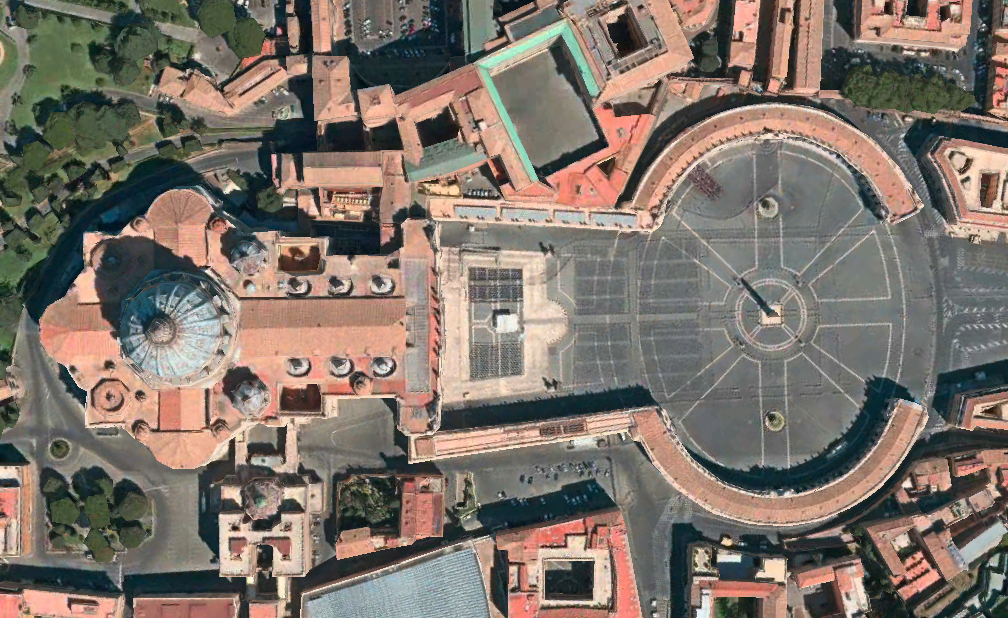
\includegraphics[width=10cm]{st-patricks-square}
		\caption{St Patrick's Square.}
	\end{figure}
\end{frame}

\begin{frame}	
	copy page over
\end{frame}

\begin{frame}[t]{Elliptic Functions}
	Arc-length of an ellipse?
\begin{equation*}
	x = a\cos\theta,\quad y=b\sin\theta\quad \quad \quad 
\end{equation*}
	
\begin{equation*}
	\begin{split}
		L &= \int_{0}^{2\pi} \sqrt{ ( \partial_{\theta}x )^{2} + ( \partial_{\theta}y )^{2} }\, d\theta \\
		&= 4a \int_{0}^{1} \sqrt{ 1 - e^{2} u^{2} }\, du \quad (e^{2} = (a^{2} - b^{2})/a^{2};\quad u = \sin\theta ) \\
		&= \frac{1}{2} \int_{1-e^{2}}^{1} \frac{t\, dt}{\sqrt{t(t-1)(t - (1-e^{2}))}}\quad (t = 1 - e^{2}u^{2})
	\end{split}
\end{equation*}	
\end{frame}

\begin{frame}[t]{Something Nicer...}
	Pendulum motion under gravity (suitable units):
	\begin{equation*}
	\dot{\theta}^{2} - \cos \theta = E,
	\end{equation*}
	with $E$ the energy and $\theta$ the amplitude angle. \\~\\
	
	Thus
	$$
		\dot{\theta} = \frac{d\theta}{dt} = \sqrt{E + \cos\theta},
	$$
	and
	\begin{equation*}
		\begin{split}
			t = \int dt = \int \frac{d\theta}{\sqrt{E + \cos \theta}} = \int \frac{du}{\sqrt{(E + u)(1 - u^{2})}}
		\end{split}
	\end{equation*}
	for $u = \cos \theta$.
\end{frame}

\begin{frame}
	Integrals of the form
	\begin{equation*}
		w = f(z) = \int_{P}^{z} \frac{dt}{ \sqrt{c_{3}t^{3} + c_{2}t^{2} + c_{1}t + c_{0}} }
	\end{equation*}
	are called \emph{elliptic integrals}. \\~\\
	
	\emph{Elliptic functions} are the inverses to elliptic integrals, $z = f^{-1}(w)$. \\~\\
	
	Analogous to $\sin^{-1}(x) = \int\frac{1}{\sqrt{1 - x^{2}}}$. \\~\\
		
	Elliptic integrals have no solution involving only elementary functions.
\end{frame}

\begin{frame}
	Denominator is a \emph{square-root} with solution set:
	\begin{equation*}
		E := \big\{ (x,y) \in \mathbb{C}^{2} :  y^{2} = x(x-1)(x-\lambda) \big\}.
	\end{equation*}
	This is called the \emph{Legendre form} of an elliptic curve. \\~\\
	
	Problem: there is no single-valued function 
	$$
	y = \pm\sqrt{f(x)} = \pm\sqrt{x(x-1)(x-\lambda)}$$
	on the whole of $\mathbb{C}$!
	
	(two sheet figure)
\end{frame}
	
\begin{frame}
	The two sheets coincide though at $x = 0, 1, \lambda$, and $\infty$. \\~\\
	
	Integrating around each of these points sends $\sqrt{f(x)} \longmapsto -\sqrt{f(x)}$. \\~\\
	
	We make $\sqrt{f(x)}$ single-valued, we glue the sheets using cuts from $0$ to $1$, and from $\lambda$ to $\infty$. \\~\\
	
	
	
	
\end{frame}

\begin{frame}	
	(Figure)
\end{frame}

\begin{frame}	
	(Figure)
\end{frame}

\begin{frame}
	Integrating $\int \frac{dx}{\sqrt{y}}$ is now well-defined up to cycles around branch cuts,
	$$
		\omega_{1} := \int_{\alpha} \frac{dx}{\sqrt{y}}, \qquad \omega_{2} := \int_{\beta} \frac{dx}{\sqrt{y}}.
	$$
	If we mod out the image of $\int \frac{dx}{\sqrt{y}}$ by $\text{Span}_{\mathbb{Z}}\{ \omega_{1}, \omega_{2} \}$, get a map
	$$
		E(\mathbb{C}) \longrightarrow \mathbb{C}/(\omega_{1}\cdot \mathbb{Z} + \omega_{2}\cdot \mathbb{Z} ).
	$$
\end{frame}

\begin{frame}[t]{The Group Law}
	Property of a cubic curve $E$: any line $L$ intersects $E$ in at most 3 points. \\~\\ 	
	
	Pick a marked point $\mathcal{O} \in E$ to serve as the identity (usually $\infty$ is chosen). \\~\\
	
	Reminder: an abelian group $G$ is a set with a binary operation $+ : G \times G \rightarrow G$ with:
	\begin{itemize}
		\item Identity, $0 \in G$;
		\item An inverse to each element, for each $g \in G$, there is a $-g \in G$;
		\item Closure, i.e. the $+$ operation does not leave the group;
		\item Associativity, i.e. $(a + b) + c = a + (b + c)$;
		\item $+$ is commutative, i.e. $a + b = b + a$.
	\end{itemize}
\end{frame}

\begin{frame}[t]{Chord and Tangent}
 	For two points $P, Q \in E$, connect them via a line $L$. This line $L$ intersects $E$ once more at a point we call $P \ast Q$. Then we define $P + Q = -(P \ast Q)$.
\end{frame}

\begin{frame}[t]{Point at Infinity}
	``\emph{Homogenise}'' the equation:
	$$
		y^{2} = x(x-1)(x-\lambda) \longmapsto y^{2}z = x(x-z)(x-\lambda z).
	$$
	i.e., introduce powers of a new coordinate $z$ so every term has degree 3. \\~\\
	
	Point at infinity obtained by setting $z = 0$, so in the above, $\infty = (0,y,0)$.
\end{frame}

\begin{frame}{Finite Fields}
	Elliptic curve addition can be defined over any field. \\~\\
	
	A field is a ``nice'' ring, \emph{e.g.} $\mathbb{Q}, \mathbb{R}, \mathbb{C}$. These are \emph{infinite fields}. \\~\\
	
	There are also \emph{finite fields}, say $\mathbb{Z}_{2}, \mathbb{Z}_{3},\ldots$. \\~\\
	
	In general $\mathbb{Z}_{p^{k}}$, with $p$ a prime number and $k\geq 1$, are all fields. \\~\\

	In $\mathbb{Z}_{p}$ arithmetic is done modulo $p$.
\end{frame}

\begin{frame}
	Elliptic curves look very different over a finite field $\mathbb{F}_{p}$!
	\begin{figure}%
		\centering
		\subfloat[$y^{2} = x^{3} + 7$ over $\mathbb{R}$]{{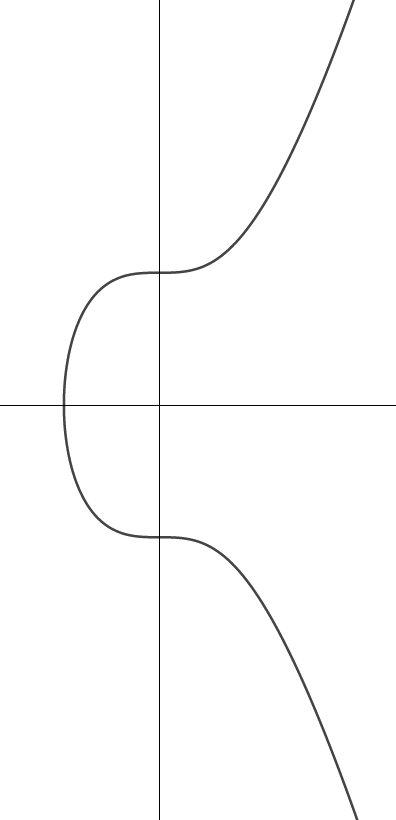
\includegraphics[height=11cm]{infinite_EC} }}%
		\qquad
		\subfloat[$y^{2} = x^{3} + 7$ over $\mathbb{F}_{13}$]{{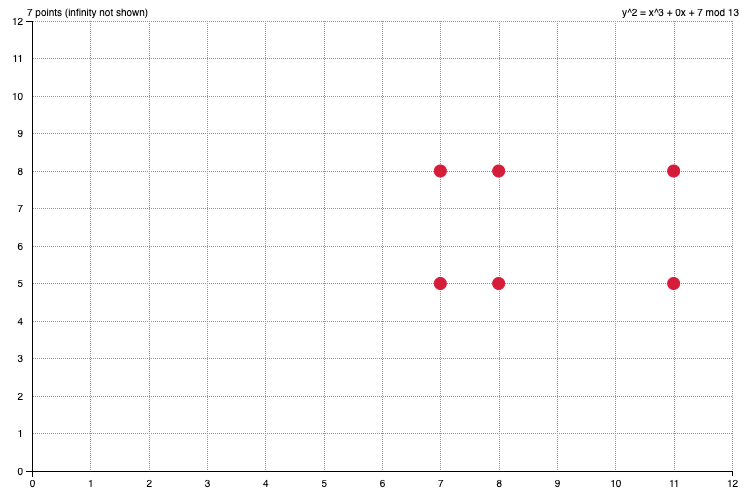
\includegraphics[width=11cm]{finite_EC-13} }}%
		\caption{Secp256k1 elliptic curve.}%
	\end{figure}
	Point $(7,5)$, we have $7^{3} + 7 = 343 + 7 = 13 \cdot 26 + 12 \equiv 12 \mod 13$, and $5^{2} = 25 \equiv 12 \mod 13$.
\end{frame}

\begin{frame}[t]{Cryptography}
	Cryptography is the process of writing using various methods, ciphers, to keep messages secret. \\~\\
	
	Example: Caesar Cipher (very insecure!) \\~\\
	\begin{itemize}
		\item ``Decrypting elliptic curves'' $\mapsto$ ``Ghfubswlqj hoolswlf fxuyhv''.
	\end{itemize}
\end{frame}

\begin{frame}[t]{Usage Cases}
	\begin{itemize}
		\item Public-Key Signatures (RSA, ECDSA); signed OS updates, SSL certificates, e-Passports.
		\item Public-Key Encryption (RSA, ECDH); SSL key exchange.
	\end{itemize}
	\begin{figure}[h]
	\centering
		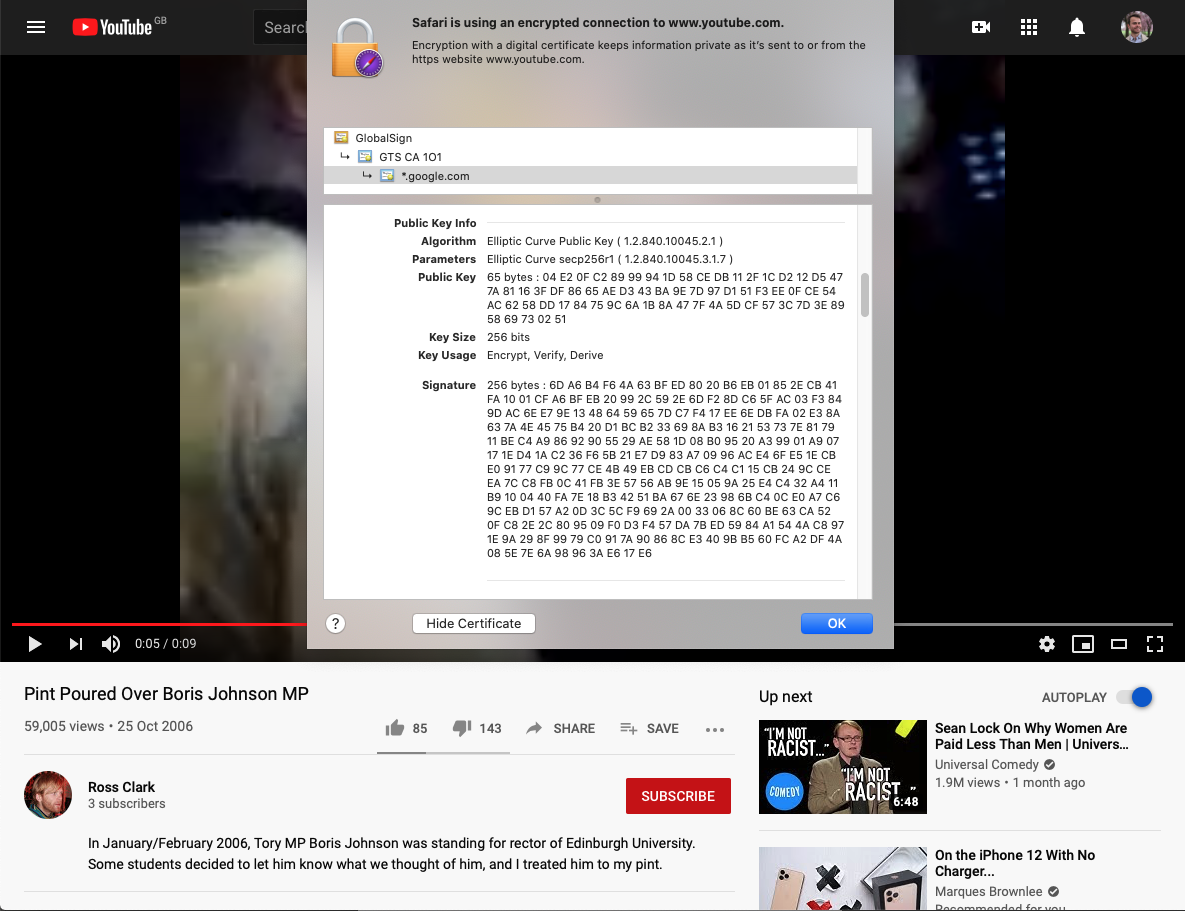
\includegraphics[width=13cm]{youtube}
		\caption{Elliptic Curve Digital Signature Algorithm.}
	\end{figure}
\end{frame}

\begin{frame}[t]{Diffie-Hellman Key Exchange}
	Standardise a large prime $p$ and base point $(x,y) \in E(\mathbb{F}_{p})$. \\~\\
	
	Alice chooses a big secret $a$, and computes her public key $a(x,y)$. \\~\\
	
	Bob chooses a big secret $b$, and computes his public key $b(x,y)$. \\~\\
	
	Alice computes $a\cdot \big(b(x,y) \big)$. \\~\\
	
	Bob computes $b \cdot \big( a(x,y)\big)$. \\~\\
	
	They use this shared secret to encrypt via a cipher.
\end{frame}

\begin{frame}
	Draw figure.
\end{frame}

\begin{frame}[t]{Discrete Logarithm Problem}
	Someone observing this exchange would only know what $E(\mathbb{F}_{p}), a(x,y), b(x,y)$ and $ab(x,y)$ are. \\~\\
	
	If we set $g = (x,y)$, Alice's public key is $g^{a} = k$. \\~\\
	
	To find her private key $a$, need to solve for
	$$
		\log_{g}k = a \mod p.
	$$
	This is the \emph{discrete logarithm problem}, and solving it is as difficult as trying a brute-force approach, i.e. trying all possible values of $a$. \\~\\\
		
\end{frame}

\begin{frame}[t]{How Long?}
	The private key $a$ can be any number in $[0,2^{256}]$, where $2^{256} \sim 1.1576 \times 10^{77}$. \\~\\
	
	That is, the size of the private key space has $10^{77}$ decimals following it. \\~\\
	
	On the other hand, the number of atoms in the visible Universe is $\sim 10^{80}$. \\~\\
	
	Elliptic curve multiplication provides a \emph{trap-door function}; easy to calculate in only one direction. \\~\\	
\end{frame}

\begin{frame}
	
\end{frame}

\end{document}
